% move all configuration stuff into one file so we can focus on the content
\documentclass[aspectratio=169,hyperref={pdfpagelabels=false,colorlinks=true,linkcolor=white,urlcolor=lightblue},xcolor={table},t]{beamer}

%%%%%%%%%%%%%%%%%%%%%%%%%%%%%%%%%%%%%%%%%%%%%%%%%%%%%%%%%%%%%%%%%%%%%%%%%%%%%%%%%%
%%%%%%%%%%%%%%%%%%%%%%%%%%%%%%%%%%%%%%%%%%%%%%%%%%%%%%%%%%%%%%%%%%%%%%%%%%%%%%%%%%
% packages
\usepackage{pict2e}
\usepackage{epic}
\usepackage{amsmath,amsfonts,amssymb}
\usepackage{units}
\usepackage{fancybox}
\usepackage[absolute,overlay]{textpos} 
%\usepackage[table]{xcolor}
\usepackage{animate}
\usepackage{gensymb}
%\usepackage{graphicx}
%\usepackage{longtable}
\usepackage{multirow}
\usepackage{silence}
\usepackage{tikz}
\usepackage[backend=bibtex,style=ieee]{biblatex}
\AtEveryCitekey{\iffootnote{\tiny}{}}
%\addbibresource{include/references}



% fontsize
\let\Tiny=\tiny

%%%%%%%%%%%%%%%%%%%%%%%%%%%%%%%%%%%%%%%%%%%%%%%%%%%%%%%%%%%%%%%%%%%%%%%%%%%%%%%%%%
%%%%%%%%%%%%%%%%%%%%%%%%%%%%%%%%%%%%%%%%%%%%%%%%%%%%%%%%%%%%%%%%%%%%%%%%%%%%%%%%%%
% warnings
\pdfsuppresswarningpagegroup=1
\WarningFilter{biblatex}{Patching footnotes failed}
\WarningFilter{latexfont}{Font shape}
\WarningFilter{latexfont}{Some font shapes}
\WarningFilter{gensymb}{Not defining}


%%%%%%%%%%%%%%%%%%%%%%%%%%%%%%%%%%%%%%%%%%%%%%%%%%%%%%%%%%%%%%%%%%%%%%%%%%%%%%%%%%
%%%%%%%%%%%%%%%%%%%%%%%%%%%%%%%%%%%%%%%%%%%%%%%%%%%%%%%%%%%%%%%%%%%%%%%%%%%%%%%%%%
% colors
\definecolor{gtgold}{rgb}{.914, .664, 0} %0e7eed {rgb}{0.88,0.66,1,0.06} [234, 170, 0]/256 %96caff
\definecolor{darkgray}{rgb}{.15, .15, .15}
\definecolor{lightblue}{HTML}{0e7eed}
\definecolor{highlight}{rgb}{0, 0, 1} %_less!40

%%%%%%%%%%%%%%%%%%%%%%%%%%%%%%%%%%%%%%%%%%%%%%%%%%%%%%%%%%%%%%%%%%%%%%%%%%%%%%%%%%
%%%%%%%%%%%%%%%%%%%%%%%%%%%%%%%%%%%%%%%%%%%%%%%%%%%%%%%%%%%%%%%%%%%%%%%%%%%%%%%%%%
% relative paths
\graphicspath{{../graph/}}


%%%%%%%%%%%%%%%%%%%%%%%%%%%%%%%%%%%%%%%%%%%%%%%%%%%%%%%%%%%%%%%%%%%%%%%%%%%%%%%%%%
%%%%%%%%%%%%%%%%%%%%%%%%%%%%%%%%%%%%%%%%%%%%%%%%%%%%%%%%%%%%%%%%%%%%%%%%%%%%%%%%%%
% units
\setlength{\unitlength}{1mm}

%%%%%%%%%%%%%%%%%%%%%%%%%%%%%%%%%%%%%%%%%%%%%%%%%%%%%%%%%%%%%%%%%%%%%%%%%%%%%%%%%%
%%%%%%%%%%%%%%%%%%%%%%%%%%%%%%%%%%%%%%%%%%%%%%%%%%%%%%%%%%%%%%%%%%%%%%%%%%%%%%%%%%
% math
\DeclareMathOperator*{\argmax}{argmax}
\DeclareMathOperator*{\argmin}{argmin}
\DeclareMathOperator*{\atan}{atan}
\DeclareMathOperator*{\arcsinh}{arcsinh}
\DeclareMathOperator*{\sign}{sign}
\DeclareMathOperator*{\tcdf}{tcdf}
\DeclareMathOperator*{\si}{sinc}
\DeclareMathOperator*{\princarg}{princarg}
\DeclareMathOperator*{\arccosh}{arccosh}
\DeclareMathOperator*{\hwr}{HWR}
\DeclareMathOperator*{\flip}{flip}
\DeclareMathOperator*{\sinc}{sinc}
\DeclareMathOperator*{\floor}{floor}
\newcommand{\e}{{e}}
\newcommand{\jom}{\mathrm{j}\omega}
\newcommand{\jOm}{\mathrm{j}\Omega}
\newcommand   {\mat}[1]    		{\boldsymbol{\uppercase{#1}}}		%bold
\renewcommand {\vec}[1]    		{\boldsymbol{\lowercase{#1}}}		%bold

%%%%%%%%%%%%%%%%%%%%%%%%%%%%%%%%%%%%%%%%%%%%%%%%%%%%%%%%%%%%%%%%%%%%%%%%%%%%%%%%%%
%%%%%%%%%%%%%%%%%%%%%%%%%%%%%%%%%%%%%%%%%%%%%%%%%%%%%%%%%%%%%%%%%%%%%%%%%%%%%%%%%%
% media9
\newcommand{\includeaudio}[1]{
\href{run:audio/#1.mp3}{
\includegraphics[width=5mm, height=5mm]{graph/SpeakerIcon}}}

\newcommand{\includeanimation}[4]{{\begin{center}
                        \animategraphics[autoplay,loop,scale=.7]{#4}{animation/#1-}{#2}{#3}        
                        \end{center}
                        \addreference{matlab source: \href{https://github.com/alexanderlerch/ACA-Plots/blob/master/matlab/animate#1.m}{matlab/animate#1.m}}}
                        \inserticon{video}}
                        
%%%%%%%%%%%%%%%%%%%%%%%%%%%%%%%%%%%%%%%%%%%%%%%%%%%%%%%%%%%%%%%%%%%%%%%%%%%%%%%%%%
%%%%%%%%%%%%%%%%%%%%%%%%%%%%%%%%%%%%%%%%%%%%%%%%%%%%%%%%%%%%%%%%%%%%%%%%%%%%%%%%%%
% other commands
\newcommand{\question}[1]{%\vspace{-4mm}
                          \setbeamercovered{invisible}
                          \begin{columns}[T]
                            \column{.9\textwidth}
                                \textbf{#1}
                            \column{.1\textwidth}
                                \vspace{-8mm}
                                \begin{flushright}
                                     
\includegraphics[width=.9\columnwidth]{graph/question_mark}
                                \end{flushright}
                                \vspace{6mm}
                          \end{columns}\pause\vspace{-12mm}}

\newcommand{\toremember}[1]{
                        \inserticon{lightbulb}
                        }

\newcommand{\matlabexercise}[1]{%\vspace{-4mm}
                          \setbeamercovered{invisible}
                          \begin{columns}[T]
                            \column{.8\textwidth}
                                \textbf{matlab exercise}: #1
                            \column{.2\textwidth}
                                \begin{flushright}
                                     \includegraphics[scale=.5]{graph/logo_matlab}
                                \end{flushright}
                                %\vspace{6mm}
                          \end{columns}}

\newcommand{\addreference}[1]{  
                  
                    \begin{textblock*}{\baselineskip }(.98\paperwidth,.5\textheight) %(1.15\textwidth,.4\textheight)
                         \begin{minipage}[b][.5\paperheight][b]{1cm}%
                            \vfill%
                             \rotatebox{90}{\tiny {#1}}
                        \end{minipage}
                   \end{textblock*}
                    }
                    
\newcommand{\figwithmatlab}[1]{
                    \begin{figure}
                        \centering
                        \includegraphics[scale=.7]{#1}
                        %\label{fig:#1}
                    \end{figure}
                    
                    \addreference{matlab source: \href{https://github.com/alexanderlerch/MUSI-6202/blob/main/matlab/plot#1.m}{plot#1.m}}}
\newcommand{\figwithref}[2]{
                    \begin{figure}
                        \centering
                        \includegraphics[scale=.7]{#1}
                        \label{fig:#1}
                    \end{figure}
                    
                    \addreference{#2}}  
                                    
\newcommand{\inserticon}[1]{
                    \begin{textblock*}{100mm}(14.5cm,7.5cm)
                        \includegraphics[height=.8cm,keepaspectratio]{graph/#1}
                    \end{textblock*}}            

%%%%%%%%%%%%%%%%%%%%%%%%%%%%%%%%%%%%%%%%%%%%%%%%%%%%%%%%%%%%%%%%%%%%%%%%%%%%%%%%%%
%%%%%%%%%%%%%%%%%%%%%%%%%%%%%%%%%%%%%%%%%%%%%%%%%%%%%%%%%%%%%%%%%%%%%%%%%%%%%%%%%%
% counters
\newcounter{i}
\newcounter{j}
\newcounter{iXOffset}
\newcounter{iYOffset}
\newcounter{iXBlockSize}
\newcounter{iYBlockSize}
\newcounter{iYBlockSizeDiv2}
\newcounter{iXBlockSizeDiv2}
\newcounter{iDistance}

\newcommand{\IEEELink}{https://ieeexplore.ieee.org/servlet/opac?bknumber=9965970}



\subtitle{Part 10: Discretization 1---Sampling}

%%%%%%%%%%%%%%%%%%%%%%%%%%%%%%%%%%%%%%%%%%%%%%%%%%%%%%%%%%%%%%%%%%%%%%%%%%%%
\begin{document}
    % generate title page
	\title[]{Digital Signal Processing for Music}   
\author[alexander lerch]{alexander lerch} 
%\institute{~}
%\date[Alexander Lerch]{}
\titlegraphic{\vspace{-16mm}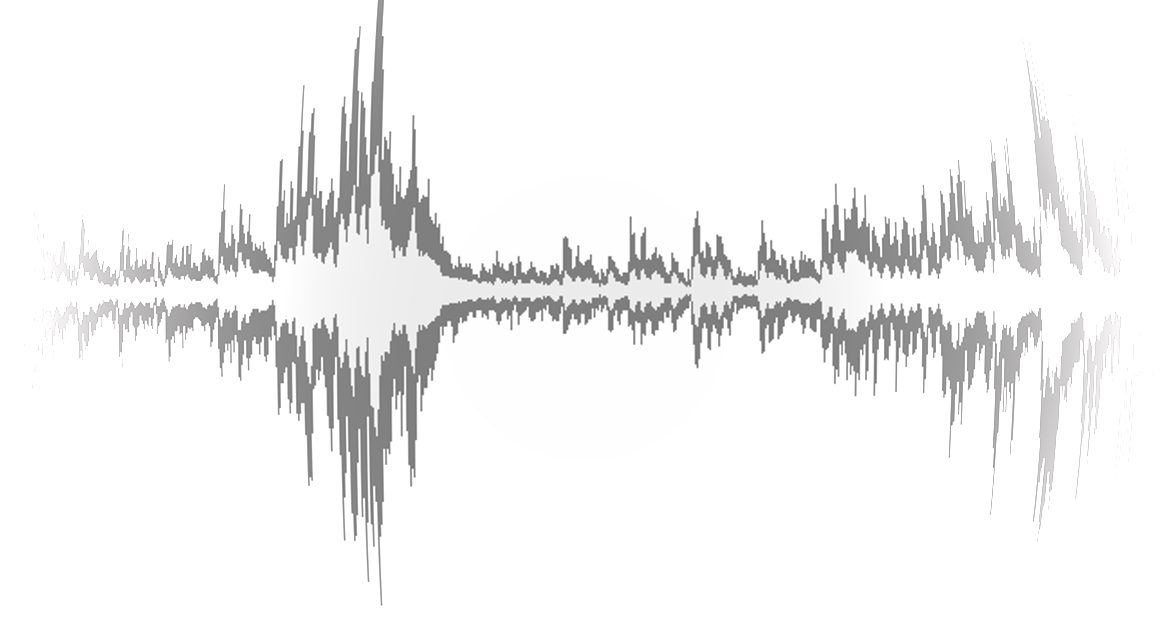
\includegraphics[width=\textwidth,height=3cm]{title}}


\begin{frame}
    \titlepage
    %\vspace{-5mm}
    \begin{flushright}
        \href{http://www.gtcmt.gatech.edu}{
\includegraphics[height=.8cm,keepaspectratio]{../shared/Logo_GTCMT_black}}
    \end{flushright}
\end{frame}


\section[intro]{introduction}
    \begin{frame}\frametitle{sampling and quantization}\framesubtitle{introduction}
        digital signals can only be represented with a limited number of values
        \pause
        
        $\Rightarrow$
        \begin{itemize}
            \item	time discretization:\\ \textbf{sampling}
            \bigskip
            \item	amplitude discretization:\\ \textbf{quantization}
        \end{itemize}
    \end{frame}
   
	\begin{frame}\frametitle{sampling and quantization}\framesubtitle{sampling}
			\vspace{-5mm}
			\begin{equation*}\nonumber
				T_{\mathrm{S}} = \frac{1}{f_{\mathrm{S}}} 
			\end{equation*}
			\begin{figure}
				\centering
					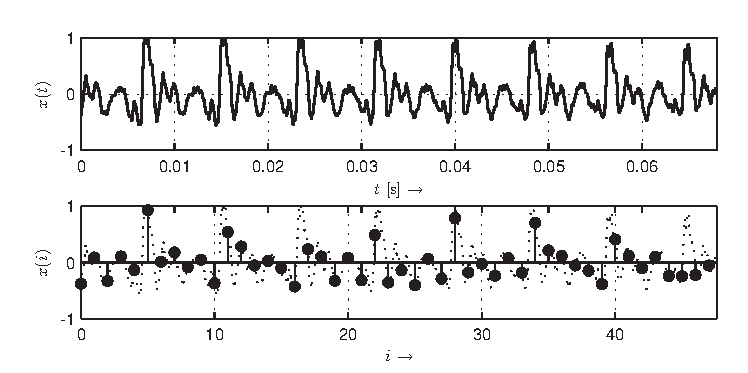
\includegraphics[scale=.6]{graph/sampling}
				\label{fig:sampling}
			\end{figure}
			\pause
            \vspace{-3mm}
			typical sample rates
			\begin{itemize}
				\item	\unit[8-16]{kHz}: speech (phone)
				\item	\unit[44.1-48]{kHz}: (consumer) audio/music
				\item	higher: production audio
			\end{itemize}
		\end{frame}	

	\section{sampling ambiguity}	
		\begin{frame}\frametitle{sampling and quantization}\framesubtitle{sampling ambiguity 1/4}
			\begin{center}
				\animategraphics[scale=.8,step]{1}{graph/samplingambi/samplingambi_}{1}{7}        
			\end{center}
			%\begin{figure}
				%\centering
					%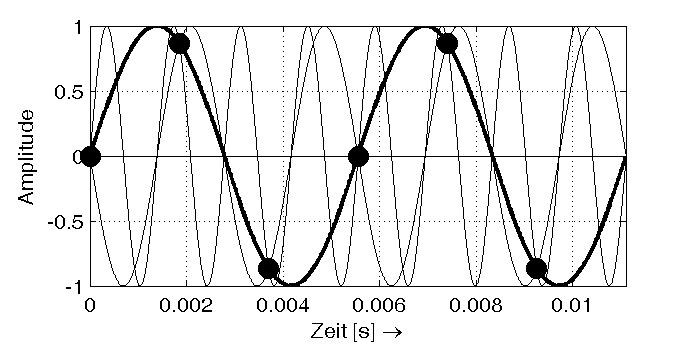
\includegraphics[scale=1.0]{Graph/sampling2}
			%\end{figure}
		\end{frame}
		
		\begin{frame}\frametitle{sampling and quantization}\framesubtitle{sampling ambiguity 2/4}
			\begin{eqnarray*}
				f_0 &=& [\unit[1, 5, 7]{kHz}]\\
				f_{\mathrm{S}} &=& \unit[6]{kHz}
			\end{eqnarray*}
			\begin{figure}
				\centering
					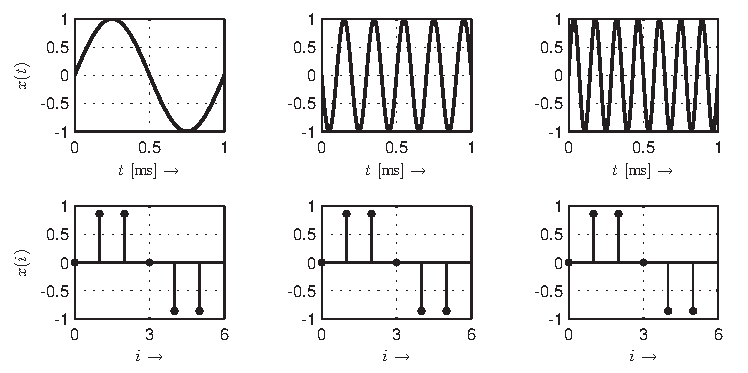
\includegraphics[scale=.7]{graph/samplingambig}
					\label{fig:samplingambig}
			\end{figure}
		\end{frame}	
		
		\begin{frame}\frametitle{sampling and quantization}\framesubtitle{sampling ambiguity 3/4}
			\textbf{wagon wheel effect}
			\invisible<2->{
			\begin{figure}
				\begin{center}
					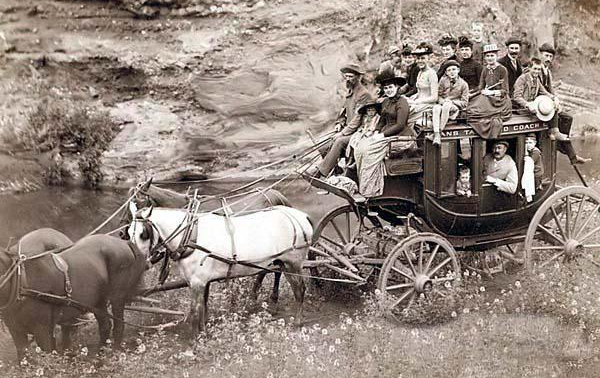
\includegraphics[scale=.4]{Graph/Stagecoach-Western}
				\end{center}
			\end{figure}
			}
			\visible<2->{
				\vspace{-60mm}
				\begin{figure}
					\begin{center}
						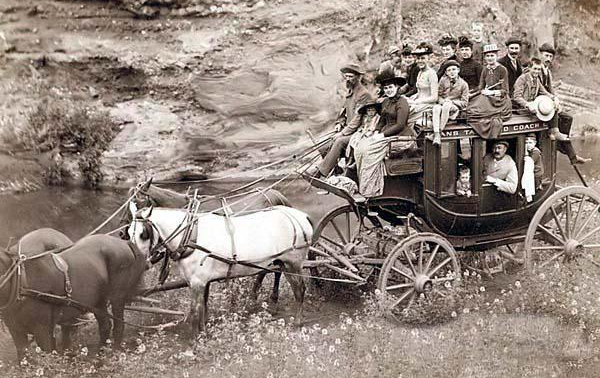
\includegraphics[scale=.2]{Graph/Stagecoach-Western}
					\end{center}
				\end{figure}
				\begin{enumerate}
					\item	$f_{wheel} < \frac{f_S}{2}$: speeding up
					\pause
					\item	$\frac{f_S}{2} < f_{wheel} < f_S$: slowing down
					\pause
					\item	$f_{wheel} = f_S$: standing still
					\pause
					\item	$\ldots$
				\end{enumerate}
			}
		\end{frame}

		\begin{frame}\frametitle{sampling and quantization}\framesubtitle{sampling ambiguity 4/4}
			\url{http://youtu.be/uENITui5_jU}
		\end{frame}	
        
        
		\begin{frame}\frametitle{sampling and quantization}\framesubtitle{sampling}
			\setbeamercovered{invisible}
            \begin{itemize}
				\item[]	$x(t) \mapsto X(\jom)$
					\vspace{-6mm}
					\uncover<1->
                    {\begin{figure}
						\flushright
							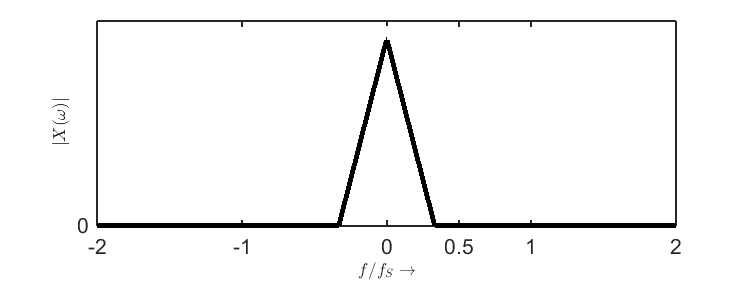
\includegraphics[scale=.4]{Graph/spectrum_sampling_1}
					\end{figure}
				}
                \pause
				\item[]	$x(t)\cdot \delta_T \mapsto X(\jom)\ast \delta_{\omega_T}$
					\vspace{-6mm}
					\uncover<2->
                    {\begin{figure}
						\flushright
							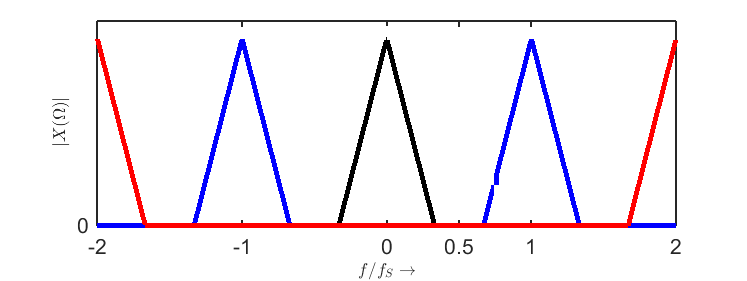
\includegraphics[scale=.4]{Graph/spectrum_sampling_2}
					\end{figure}
                    }
			\end{itemize}		
            \uncover<3->{
			\begin{center}
				\animategraphics[scale=.5,autoplay,loop]{10}{graph/SpectralAliasing/aliasing_}{1}{101}        
			\end{center}
            }
		\end{frame}
		
	\section{sampling theorem}	
		\begin{frame}\frametitle{sampling and quantization}\framesubtitle{sampling theorem}
			\toremember{}
			\begin{block}{sampling theorem}
				\centering
				A sampled audio signal can  be reconstructed \textbf{without loss of information} if the sample rate $f_{\mathrm{S}}$ is higher than twice the bandwidth $f_{\mathrm{max}}$  of the signal.
				\begin{equation*}\label{eq:sample_theorem}	
					f_{\mathrm{S}} > 2\cdot f_{\mathrm{max}}
				\end{equation*}
			\end{block}
			%\begin{quote}
				 %``The intuitive justification is that, if x(t) contains no frequencies higher than \nicefrac{f_\mathrm{max}, it cannot change to a substantially new value in a time less than one-half cycle of the highest frequency".
			%\end{quote}
		\end{frame}
		
	\section{aliasing}	
		\begin{frame}\frametitle{sampling and quantization}\framesubtitle{sampling: aliasing}
			\begin{figure}
				\begin{center}
					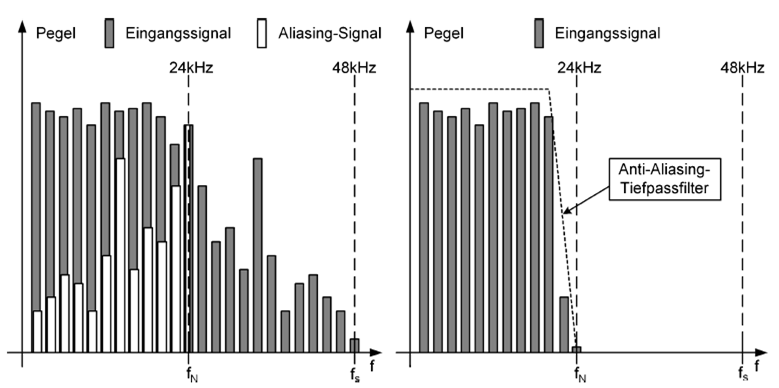
\includegraphics[scale=0.5]{Graph/aliasing}
				\end{center}
			\end{figure} 
		\end{frame}	

		\begin{frame}\frametitle{sampling and quantization}\framesubtitle{sampling: aliasing examples 1/2}
			\vspace{-3mm}
			audio example: sinesweep 100--10k at 24, 12, 6k
            \vspace{-3mm}
			\begin{columns}
				\column{.7\textwidth}
				\vspace{-5mm}
				\begin{figure}
					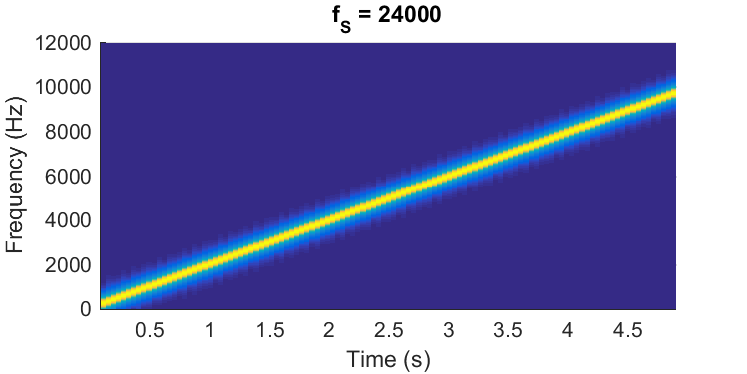
\includegraphics[scale=.35]{graph/sinealiasing_1}
				\end{figure}
				\visible<2->{
				\vspace{-8mm}
				\begin{figure}
					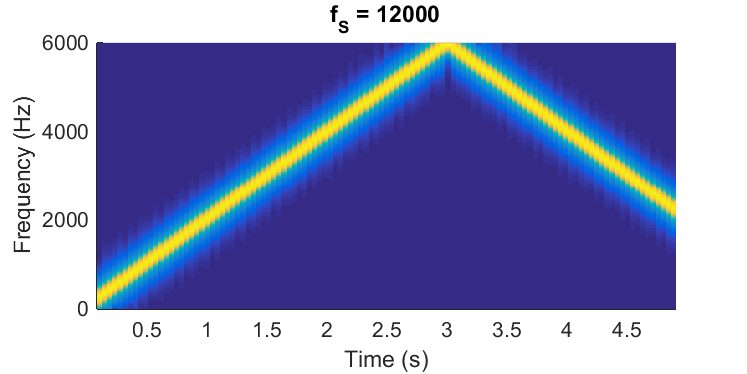
\includegraphics[scale=.35]{graph/sinealiasing_2}
				\end{figure}
				}
				\visible<3->{
				\vspace{-8mm}
				\begin{figure}
					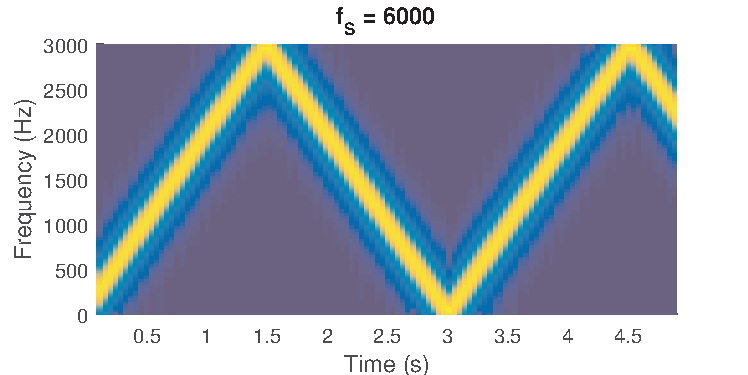
\includegraphics[scale=.35]{graph/sinealiasing_3}
				\end{figure}
				}
				\column{.3\textwidth}
				
				\includeaudio{sinealiasing_1}
				%\begin{figure}
					%
\includegraphics[scale=.05]{graph/SpeakerIcon}
				%\end{figure}
				%\vspace{-3mm}
				%sinealiasing\_1.wav
				\bigskip
				\bigskip
				\bigskip
				\bigskip
				\bigskip
				
				\visible<2->{
				\includeaudio{sinealiasing_2}
				%\begin{figure}
					%
\includegraphics[scale=.05]{graph/SpeakerIcon}
				%\end{figure}
				%\vspace{-3mm}
				%sinealiasing\_2.wav
				\bigskip
				\bigskip
				\bigskip
				\bigskip
				\bigskip
			   }
				
				\visible<3->{
				\includeaudio{sinealiasing_3}
				%\begin{figure}
					%
\includegraphics[scale=.05]{graph/SpeakerIcon}
				%\end{figure}
				%\vspace{-3mm}
				%sinealiasing\_3.wav
				}
			\end{columns}
			%\begin{itemize}
				%\item	original (\unit[44.1]{kHz})
						%\begin{figure}
							%\includemovie[poster=graph/SpeakerIcon.png,mouse=true]{1cm}{1cm}{audio/bigband.wav}
						%\end{figure}
				%\item	downsampled (\unit[11.025]{kHz}) \textit{without} aliasing filter
						%\begin{figure}
							%\includemovie[poster=graph/SpeakerIcon.png,mouse=true]{1cm}{1cm}{audio/bigbandds.wav}
						%\end{figure}
				%\item	downsampled (\unit[11.025]{kHz}) \textit{with} aliasing filter
						%\begin{figure}
							%\includemovie[poster=graph/SpeakerIcon.png,mouse=true]{1cm}{1cm}{audio/bigbandds_proper.wav}
						%\end{figure}
			%\end{itemize}
		\end{frame}	

		\begin{frame}\frametitle{sampling and quantization}\framesubtitle{sampling: aliasing examples 2/2}
            \setbeamercovered{invisible}
            \begin{itemize}
                \item \textbf{bigband}
                \begin{itemize}
                    \item   original (\unit[48]{kHz}): \includeaudio{bigband}
                    \item   samples discarded (\unit[6]{kHz}): \includeaudio{bigbandds8}
                    \item   downsampling  w/ anti-aliasing filter (\unit[6]{kHz}): \includeaudio{bigbandds8_proper}
                \end{itemize}
                \pause
                \bigskip
                \item   \textbf{sax}
                \begin{itemize}
                    \item   original (\unit[48]{kHz}): \includeaudio{alto-sax}
                    \item   samples discarded (\unit[6]{kHz}): \includeaudio{alto-saxds8}
                    \item   downsampling w/ anti-aliasing filter (\unit[6]{kHz}): \includeaudio{alto-saxds8_proper}
                \end{itemize}
            \end{itemize}
		\end{frame}

	\section{summary}	
		\begin{frame}{sampling and quantization}{sampling: summary 1/2}
			\begin{enumerate}
				\item[]   continuous input signal
                \item[] \hspace{10mm}$\downarrow$
				\pause
				\item   \textbf{anti-aliasing filter}
				\pause
                \smallskip
				\item[] filtered continuous input signal
				\pause
				\item   \textbf{sampling}
				\pause
                \smallskip
				\item[] sampled input signal
				\pause
                \smallskip
				\item   \textbf{reconstruction filter}
				\pause
                \item[] \hspace{10mm}$\downarrow$
				\item[] continuous output signal
			\end{enumerate}
		\end{frame}
 
		\begin{frame}{sampling and quantization}{sampling: summary 2/2}
			\begin{itemize}
				\item   sampling theorem
                    \begin{quote}
                        A sampled audio signal can be reconstructed without loss of information if the sample rate $f_\mathrm{S}$ is higher than twice the bandwidth f max of the signal.
                    \end{quote}
                    \begin{itemize}
                        \item   perfect reconstruction!
                        \item   ensure accordance through filtering, otherwise aliasing (mirror frequencies)
                    \end{itemize}
                \item   band of interest does not have to be base band ($0\ldots f_\mathrm{S}/2$), but any band ($k\cdot f_\mathrm{S}/2\ldots(k+1)\cdot f_\mathrm{S}/2$) as long as the bandwidth is not wider 
			\end{itemize}
		\end{frame}

\end{document}

